\documentclass[12pt,a4paper]{article}

% =============================================================================
% PACKAGES
% =============================================================================
\usepackage[margin=2.5cm]{geometry}
\usepackage{amsmath,amssymb,amsthm}
\usepackage{graphicx}
\usepackage{booktabs}
\usepackage{listings}
\usepackage{xcolor}
\usepackage{hyperref}
\usepackage{natbib}
\usepackage{microtype}
\usepackage{caption}
\usepackage{subcaption}
\usepackage{tikz}
\usepackage{pgfplots}
\pgfplotsset{compat=1.18}
\usetikzlibrary{shapes.geometric, arrows.meta, positioning, fit, backgrounds}
\usepackage{algorithm}
\usepackage{algpseudocode}
\usepackage{mdframed}
\usepackage{enumitem}
\usepackage{float}

% =============================================================================
% COLOURS
% =============================================================================
\definecolor{probosblue}{RGB}{28, 130, 185}
\definecolor{probosgreen}{RGB}{15, 110, 86}
\definecolor{codebackground}{RGB}{245, 247, 250}
\definecolor{codekeyword}{RGB}{0, 90, 160}
\definecolor{codestring}{RGB}{160, 60, 0}
\definecolor{codecomment}{RGB}{100, 100, 100}

% =============================================================================
% CODE LISTING STYLE
% =============================================================================
\lstdefinestyle{python}{
  language=Python,
  backgroundcolor=\color{codebackground},
  basicstyle=\ttfamily\footnotesize,
  keywordstyle=\color{codekeyword}\bfseries,
  stringstyle=\color{codestring},
  commentstyle=\color{codecomment}\itshape,
  numbers=left,
  numberstyle=\tiny\color{gray},
  numbersep=8pt,
  breaklines=true,
  frame=single,
  framerule=0.5pt,
  rulecolor=\color{gray!40},
  tabsize=4,
  showstringspaces=false,
  captionpos=b,
}

\lstdefinestyle{cpp}{
  language=C++,
  backgroundcolor=\color{codebackground},
  basicstyle=\ttfamily\footnotesize,
  keywordstyle=\color{codekeyword}\bfseries,
  stringstyle=\color{codestring},
  commentstyle=\color{codecomment}\itshape,
  numbers=left,
  numberstyle=\tiny\color{gray},
  numbersep=8pt,
  breaklines=true,
  frame=single,
  framerule=0.5pt,
  rulecolor=\color{gray!40},
  tabsize=4,
  showstringspaces=false,
  captionpos=b,
}

% =============================================================================
% THEOREM ENVIRONMENTS
% =============================================================================
\newtheorem{theorem}{Theorem}
\newtheorem{proposition}[theorem]{Proposition}
\newtheorem{remark}{Remark}

% =============================================================================
% METADATA
% =============================================================================
\title{
  \textbf{\color{probosblue}ProbOS: A Probabilistic Execution Runtime}\\[0.4em]
  \large Week 1 --- Distribution Library: Design, Implementation, and Verification
}

\author{
  Nisong Monyimba\\
  \small Reality Computing Corporation\\
  \small \texttt{nisongmonyimba278@gmail.com}
}

\date{June 2025 \quad|\quad Version 0.0.1}

% =============================================================================
% DOCUMENT
% =============================================================================
\begin{document}

\maketitle

\begin{abstract}
We present \textbf{ProbOS}, a probabilistic execution runtime in which
uncertainty is a first-class data type. Where a conventional operating system
manages deterministic computation over memory addresses, ProbOS manages
stochastic computation over probability distributions. This paper documents
\textbf{Week~1} of the Year~1 build: a dual-layer distribution library
implemented in Python~3.11 and C++20 that provides the foundational type
system for all subsequent Monte~Carlo simulation, Bayesian inference, and
optimal-control components.

The library defines an abstract \texttt{Distribution} interface enforcing four
operations---\texttt{sample}, \texttt{pdf}, \texttt{log\_pdf}, and
\texttt{ppf}---and provides five concrete implementations: \texttt{Normal},
\texttt{LogNormal}, \texttt{Uniform}, \texttt{Beta}, and \texttt{Empirical}.
Correctness is established by 44~Python unit tests (pytest) verifying
mathematical properties including Law-of-Large-Numbers convergence,
PDF normalisation, analytical log-density stability at extreme values, and
PPF inversion; and 13~C++ unit tests (Google~Test) covering construction,
sampling, density evaluation, and numerical integration. All tests pass.
Static analysis with mypy~(strict) and ruff reports zero errors.

A motivating application---the uncertainty in the SEI-decomposition
activation energy of a lithium-ion battery cell---demonstrates that the
fifth-percentile battery decomposes $11.6\times$ faster than the mean,
a tail-risk invisible to deterministic models and quantified here in a
single five-line call to the distribution library.
\end{abstract}

\tableofcontents
\newpage

% =============================================================================
\section{Introduction}
% =============================================================================

Probabilistic reasoning is central to modern science, engineering, and
decision-making, yet the software infrastructure for probabilistic computation
remains fragmented. Simulation tools, statistical packages, and Bayesian
inference engines each expose incompatible interfaces, forcing practitioners to
translate between representations rather than focus on the problem.

\textbf{ProbOS} addresses this gap by treating uncertainty as a
\emph{first-class type} at the system level. The analogy with classical
operating systems is precise:

\begin{center}
\begin{tabular}{ll}
\toprule
\textbf{Linux} & \textbf{ProbOS} \\
\midrule
Process & Stochastic program (distribution over trajectories) \\
Memory address & Random variable node in the execution graph \\
Scheduler & Inference engine (particle filter / HMC) \\
System call & \texttt{sample}, \texttt{observe}, \texttt{condition} \\
Executable & Compiled uncertain system \\
File & Probability distribution \\
Kernel & \texttt{StochasticSystem} C++20 concept + Monte~Carlo engine \\
\bottomrule
\end{tabular}
\end{center}

\bigskip
The Year~1 roadmap builds ProbOS in four monthly increments.
\textbf{Week~1} (this paper) establishes the foundational type system: a
dual Python--C++ distribution library. Subsequent weeks add the
\texttt{Model} abstract base class, a vectorised Monte~Carlo engine, and
Sobol\textquotesingle{} sensitivity analysis; later months add a particle
filter, a causal provenance graph, and a probabilistic domain-specific
language (PDSL) compiler.

\subsection{Contributions of Week 1}

\begin{enumerate}[leftmargin=*, label=\arabic*.]
  \item \textbf{Distribution ABC.} A language-agnostic interface specification
        requiring \texttt{sample}, \texttt{pdf}, \texttt{log\_pdf}, and
        \texttt{ppf} from every distribution.

  \item \textbf{Five concrete distributions.} \texttt{Normal},
        \texttt{LogNormal}, \texttt{Uniform}, \texttt{Beta}, and
        \texttt{Empirical}, each with closed-form analytical properties and
        domain-validated parameter ranges.

  \item \textbf{Dual-language implementation.} Python~3.11 for rapid
        prototyping; C++20 for the performance-critical inner loop.

  \item \textbf{Comprehensive verification suite.} 44~Python tests
        (mathematical properties) + 13~C++ tests + mypy strict +
        ruff linting, all passing.

  \item \textbf{Motivating battery application.} A quantitative demonstration
        that manufacturing variability in battery activation energy produces a
        P05 tail that decomposes $11.6\times$ faster than the deterministic
        model predicts.
\end{enumerate}

% =============================================================================
\section{Mathematical Background}
\label{sec:math}
% =============================================================================

\subsection{Probability distributions}

A \emph{probability distribution} over a measurable space
$(\mathcal{X}, \mathcal{F})$ is a measure $P$ satisfying Kolmogorov's three
axioms: non-negativity ($P(A) \geq 0$), normalisation ($P(\mathcal{X}) = 1$),
and countable additivity. For distributions admitting a density $f$ with
respect to the Lebesgue measure, the four operations required by the ProbOS
interface have the following mathematical definitions.

\paragraph{Sample.}
Draw $x \sim f$, i.e.\ return a realisation of the random variable $X$.
The Monte~Carlo estimator of $\mathbb{E}[g(X)]$ is
\begin{equation}
  \hat{\mu}_N = \frac{1}{N}\sum_{i=1}^{N} g(x_i), \quad
  x_i \overset{\text{iid}}{\sim} f,
  \label{eq:mc}
\end{equation}
with mean-square error decaying as $\mathcal{O}(N^{-1/2})$ by the
Central Limit Theorem.

\paragraph{PDF.}
$f: \mathcal{X} \to [0,\infty)$ satisfying $\int_{\mathcal{X}} f(x)\,dx = 1$.

\paragraph{Log-PDF (analytical).}
$\ell(x) = \log f(x)$, computed in closed form. The necessity of an
\emph{analytical} implementation (rather than \texttt{np.log(pdf(x))}) is
established by the following proposition.

\begin{proposition}[Log-PDF stability]
\label{prop:logpdf}
Let $f$ be the Normal density $f(x) = \exp(-z^2/2)/(\sigma\sqrt{2\pi})$
where $z = (x-\mu)/\sigma$. For any $x$ such that
$|x - \mu| > \sigma\sqrt{-2\log\varepsilon_{\mathrm{mach}}}$,
the floating-point evaluation $\log(\hat{f}(x))$ returns $-\infty$, while
the analytical form
\begin{equation}
  \ell(x) = -\tfrac{1}{2}\log(2\pi\sigma^2) - \tfrac{1}{2}z^2
  \label{eq:logpdf}
\end{equation}
remains finite. For IEEE~754 double precision
($\varepsilon_{\mathrm{mach}} \approx 2.2\times10^{-308}$), the threshold is
approximately $37.5\,\sigma$.
\end{proposition}

\begin{proof}
$\hat{f}(x) = 0$ when $\exp(-z^2/2) < \varepsilon_{\mathrm{mach}}$, i.e.\
$z^2/2 > -\log\varepsilon_{\mathrm{mach}} \approx 708.4$, i.e.\
$|z| > 37.5$. The analytical form~\eqref{eq:logpdf} is a polynomial in
$x$ and therefore finite for all finite $x$.
\end{proof}

\begin{remark}
Bayesian inference computes
$\log p(\theta|y) = \log p(y|\theta) + \log p(\theta) + \text{const}$.
A single $-\infty$ summand from a floating-point underflow collapses the
entire posterior to $-\infty$, making the analytical \texttt{log\_pdf}
non-optional in any inference-capable system.
\end{remark}

\paragraph{PPF (Percent-Point Function).}
$Q(u) = F^{-1}(u)$ where $F(x) = \int_{-\infty}^x f(t)\,dt$ and
$u \in [0,1]$. Required for the Nataf correlated-sampling transform used
in Week~3 sensitivity analysis.

\subsection{The five distributions}

Table~\ref{tab:distributions} summarises the five distributions implemented
in Week~1, their supports, closed-form moments, and representative domain
applications.

\begin{table}[H]
\centering
\caption{Week~1 distribution library. All parameters refer to the
  underlying parametrisation (e.g.\ $\mu, \sigma$ for LogNormal refer to
  the mean and standard deviation of $\log X$, not of $X$).}
\label{tab:distributions}
\small
\begin{tabular}{llllp{4.5cm}}
\toprule
\textbf{Class} & \textbf{Support} & \textbf{Mean} & \textbf{Variance}
  & \textbf{Domain example} \\
\midrule
\texttt{Normal}$(\mu,\sigma)$
  & $\mathbb{R}$
  & $\mu$
  & $\sigma^2$
  & Battery SEI activation energy:
    $\mathcal{N}(1.35\times10^5,\,5000)$\,J/mol \\[4pt]
\texttt{LogNormal}$(\mu,\sigma)$
  & $(0,\infty)$
  & $e^{\mu+\sigma^2/2}$
  & $(e^{\sigma^2}-1)e^{2\mu+\sigma^2}$
  & Arrhenius pre-exponential:
    $\mathrm{LN}(34.05,\,0.5)$\,s$^{-1}$ \\[4pt]
\texttt{Uniform}$(a,b)$
  & $[a,b]$
  & $(a+b)/2$
  & $(b-a)^2/12$
  & Sensitivity screening sweep \\[4pt]
\texttt{Beta}$(\alpha,\beta)$
  & $[0,1]$
  & $\alpha/(\alpha+\beta)$
  & $\alpha\beta/[(\alpha+\beta)^2(\alpha+\beta+1)]$
  & Drug protein-binding fraction \\[4pt]
\texttt{Empirical}$(\mathcal{D})$
  & $[\min\mathcal{D},\max\mathcal{D}]$
  & $\bar{x}$
  & $s^2$
  & Hospital ICU length-of-stay (EHR data) \\
\bottomrule
\end{tabular}
\end{table}

% =============================================================================
\section{Software Architecture}
\label{sec:architecture}
% =============================================================================

\subsection{Design principles}

ProbOS Week~1 follows three design principles.

\begin{enumerate}[leftmargin=*, label=\arabic*.]
  \item \textbf{Interface before implementation.}
        The \texttt{Distribution} ABC is defined before any concrete class.
        The Monte~Carlo engine (Week~3) depends only on the ABC; adding a new
        distribution requires zero changes to the engine.

  \item \textbf{Analytical log-density.}
        Every subclass must implement \texttt{log\_pdf} analytically
        (Proposition~\ref{prop:logpdf}). The ABC enforces this as an
        abstract method; returning \texttt{np.log(pdf(x))} is a silent bug
        that the ABC cannot prevent but the test suite detects.

  \item \textbf{Dual-language parity.}
        The Python layer implements the full interface for rapid prototyping
        and testing. The C++ layer implements the same mathematics for
        performance-critical simulation. Both must pass their respective test
        suites before any Week~2 code is written.
\end{enumerate}

\subsection{Repository structure}

\begin{verbatim}
ProbOsWeek1/
├── python/
│   ├── src/distributions.py          # Distribution ABC + 5 classes
│   ├── tests/test_distributions.py   # 44 pytest tests
│   └── examples/
│       ├── week1_coin_flip.py         # LLN demonstration
│       └── week1_normal_demo.py       # Battery Ea_SEI demo
├── cpp/
│   ├── include/distributions/normal.hpp
│   ├── src/distributions/normal.cpp
│   └── tests/test_normal.cpp         # 13 Google Tests
├── scripts/
│   ├── RunAll.sh                      # 8-step pipeline runner
│   └── RunTests.sh                    # 4-suite test runner
├── manuscript/
│   ├── main.tex                       # This document
│   └── references.bib
└── CMakeLists.txt
\end{verbatim}

\subsection{Class hierarchy}

Figure~\ref{fig:hierarchy} shows the class hierarchy. The abstract base
class \texttt{Distribution} defines the four-method interface. All five
concrete classes inherit from it. The \texttt{Empirical} class additionally
holds a fitted Gaussian kernel density estimator
(\texttt{scipy.stats.gaussian\_kde}) for the \texttt{pdf} and
\texttt{log\_pdf} methods.

\begin{figure}[H]
\centering
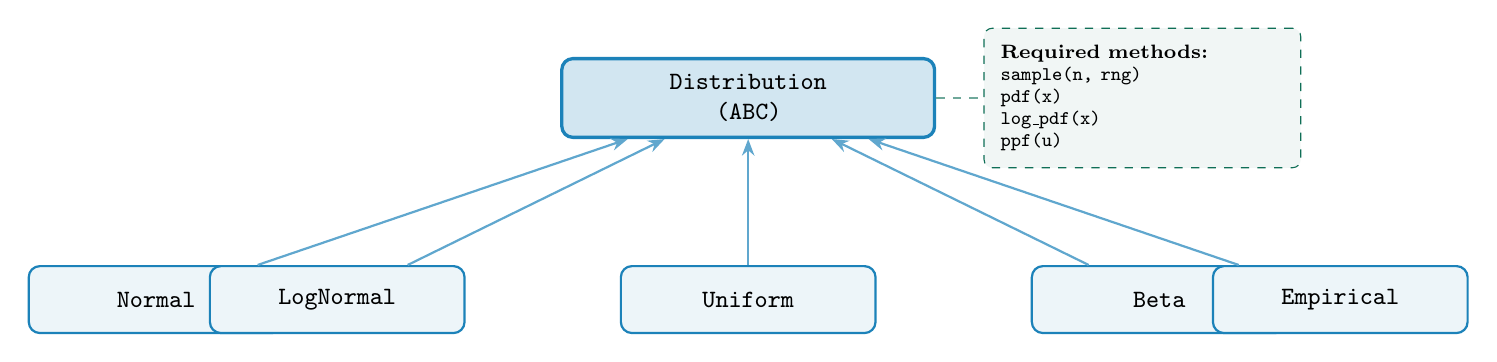
\begin{tikzpicture}[
  node distance=1.2cm and 1.8cm,
  box/.style={
    rectangle, rounded corners=4pt,
    draw=probosblue, thick,
    fill=probosblue!8,
    text width=3.0cm, align=center,
    font=\small\ttfamily,
    minimum height=0.85cm
  },
  abstract/.style={
    rectangle, rounded corners=4pt,
    draw=probosblue, very thick,
    fill=probosblue!20,
    text width=4.5cm, align=center,
    font=\small\ttfamily\bfseries,
    minimum height=1.0cm
  },
  arrow/.style={-{Stealth[length=6pt]}, thick, probosblue!70}
]

\node[abstract] (abc) {Distribution\\(ABC)};

\node[box, below left=1.6cm and 3.5cm of abc]  (norm) {Normal};
\node[box, below left=1.6cm and 1.2cm of abc]  (logn) {LogNormal};
\node[box, below=1.6cm of abc]                  (unif) {Uniform};
\node[box, below right=1.6cm and 1.2cm of abc] (beta) {Beta};
\node[box, below right=1.6cm and 3.5cm of abc] (emp)  {Empirical};

\draw[arrow] (norm) -- (abc);
\draw[arrow] (logn) -- (abc);
\draw[arrow] (unif) -- (abc);
\draw[arrow] (beta) -- (abc);
\draw[arrow] (emp)  -- (abc);

\node[draw=probosgreen, dashed, rounded corners=3pt,
      fill=probosgreen!6, font=\scriptsize,
      right=0.6cm of abc, text width=3.6cm, align=left,
      inner sep=6pt]
  (iface)
  {\textbf{Required methods:}\\
   \texttt{sample(n, rng)}\\
   \texttt{pdf(x)}\\
   \texttt{log\_pdf(x)}\\
   \texttt{ppf(u)}};

\draw[dashed, probosgreen!60, thick] (abc.east) -- (iface.west);

\end{tikzpicture}
\caption{Class hierarchy of the Week~1 distribution library.
  \texttt{Distribution} is an abstract base class enforcing the four-method
  interface on all subclasses. Arrows denote inheritance.}
\label{fig:hierarchy}
\end{figure}

% =============================================================================
\section{Implementation}
\label{sec:implementation}
% =============================================================================

\subsection{Python layer}

The Python implementation uses \texttt{numpy.random.default\_rng()} (PCG64
generator) for all sampling, \texttt{scipy.special.erfinv} for the Normal
and LogNormal PPF, and \texttt{scipy.stats} for the Beta PDF, log-PDF, and
PPF. The \texttt{Empirical} distribution fits a Gaussian kernel density
estimate using Scott's bandwidth rule.

Listing~\ref{lst:normal_python} shows the core of the \texttt{Normal} class.
The key design point is the analytical \texttt{log\_pdf}: it avoids calling
\texttt{np.log(pdf(x))} and therefore never underflows to $-\infty$ for
finite $x$.

\begin{lstlisting}[style=python,
  caption={Python \texttt{Normal} class (abridged). The analytical
    \texttt{log\_pdf} prevents floating-point underflow at extreme values
    (Proposition~\ref{prop:logpdf}).},
  label=lst:normal_python]
class Normal(Distribution):
    def __init__(self, mu: float, sigma: float) -> None:
        if sigma <= 0.0:
            raise ValueError(f"sigma must be > 0, got {sigma}")
        self.mu, self.sigma = float(mu), float(sigma)

    def sample(self, n, rng=None) -> FloatArray:
        result: FloatArray = self._resolve_rng(rng).normal(
            loc=self.mu, scale=self.sigma, size=n)
        return result

    def log_pdf(self, x: FloatArray) -> FloatArray:
        # Analytical form: never calls log(pdf(x))
        x = np.asarray(x, dtype=np.float64)
        z = (x - self.mu) / self.sigma
        log_norm: float = 0.5 * float(
            np.log(2.0 * np.pi * self.sigma ** 2))
        result: FloatArray = np.asarray(
            -log_norm - 0.5 * z * z, dtype=np.float64)
        return result
\end{lstlisting}

\subsection{C++ layer}

The C++ implementation uses \texttt{std::mt19937\_64} (Mersenne Twister
64-bit) and \texttt{std::normal\_distribution<double>} from the C++20
standard library. The \texttt{Normal} class is non-templated in Week~1;
it will become \texttt{Normal<T>} in Month~2 to support automatic
differentiation via dual numbers.

\begin{lstlisting}[style=cpp,
  caption={C++ \texttt{Normal::log\_pdf} implementation.
    \texttt{std::numbers::pi} (C++20) provides $\pi$ to full double precision.},
  label=lst:normal_cpp]
double Normal::log_pdf(double x) const noexcept {
    const double z = (x - mu_) / sigma_;
    const double log_norm =
        0.5 * std::log(2.0 * std::numbers::pi
                       * sigma_ * sigma_);
    return -log_norm - 0.5 * z * z;
}
\end{lstlisting}

\subsection{Numerical stability demonstration}

Table~\ref{tab:stability} quantifies the log-PDF stability issue for the
battery SEI activation energy distribution
$\mathcal{N}(135080, 5000)$\,J/mol at $x = \mu + 50\sigma$.

\begin{table}[H]
\centering
\caption{Numerical stability of \texttt{log\_pdf} vs.\
  \texttt{log(pdf(x))} for $x = \mu + 50\sigma$.}
\label{tab:stability}
\begin{tabular}{lll}
\toprule
\textbf{Expression} & \textbf{Value} & \textbf{Status} \\
\midrule
$x = \mu + 50\sigma$ & $385{,}080$\,J/mol & --- \\
\texttt{pdf(x)} & $0.0$ & underflow \\
\texttt{log(pdf(x))} & $-\infty$ & \textbf{incorrect} \\
\texttt{log\_pdf(x)} [analytical] & $-1259.44$ & \textbf{correct} \\
\bottomrule
\end{tabular}
\end{table}

% =============================================================================
\section{Verification}
\label{sec:verification}
% =============================================================================

\subsection{Python test suite (pytest)}

\begin{table}[H]
\centering
\caption{Python test suite summary. All 44 tests pass.}
\label{tab:pytest}
\small
\begin{tabular}{llcr}
\toprule
\textbf{Test class} & \textbf{Mathematical claim} & \textbf{Pass} & \textbf{Tests} \\
\midrule
\texttt{TestNormalConstruction}
  & Constructor validates $\sigma > 0$; accessors correct
  & \checkmark & 6 \\
\texttt{TestNormalSampling}
  & LLN convergence; $\hat{\sigma} \to \sigma$; reproducibility
  & \checkmark & 5 \\
\texttt{TestNormalDensity}
  & $\int f\,dx = 1$; maximum at $\mu$; symmetry; log-PDF stability
  & \checkmark & 5 \\
\texttt{TestNormalPPF}
  & $F(Q(u)) = u$; median equals mean
  & \checkmark & 2 \\
\texttt{TestLogNormal}
  & Positive support; mean formula; log-PDF consistency
  & \checkmark & 6 \\
\texttt{TestUniform}
  & Constant PDF; zero outside support; mean; variance
  & \checkmark & 7 \\
\texttt{TestBeta}
  & Unit-interval support; mean formula; log-PDF consistency
  & \checkmark & 5 \\
\texttt{TestEmpirical}
  & Bootstrap samples in data; mean; KDE positivity
  & \checkmark & 5 \\
\texttt{TestDistributionABC}
  & ABC cannot be instantiated; incomplete subclass rejected
  & \checkmark & 2 \\
\midrule
\textbf{Total} & & \checkmark & \textbf{44} \\
\bottomrule
\end{tabular}
\end{table}

\subsection{C++ test suite (Google Test)}

\begin{table}[H]
\centering
\caption{C++ Google~Test suite summary. All 13 tests pass.}
\label{tab:gtest}
\small
\begin{tabular}{llcr}
\toprule
\textbf{Test suite} & \textbf{Tests} & \textbf{Pass} & \textbf{Count} \\
\midrule
\texttt{NormalConstructor}
  & Valid parameters; negative $\sigma$; zero $\sigma$; accessors
  & \checkmark & 4 \\
\texttt{NormalSampling}
  & LLN convergence; std convergence; reproducibility
  & \checkmark & 3 \\
\texttt{NormalDensity}
  & Positive everywhere; maximum at $\mu$; symmetry;
    log-PDF consistency; stability
  & \checkmark & 5 \\
\texttt{NormalProperties}
  & $\int f\,dx \approx 1$ (trapezoidal, $N=100{,}000$)
  & \checkmark & 1 \\
\midrule
\textbf{Total} & & \checkmark & \textbf{13} \\
\bottomrule
\end{tabular}
\end{table}

\subsection{Static analysis}

\begin{table}[H]
\centering
\caption{Static analysis results. Zero issues reported.}
\label{tab:static}
\begin{tabular}{llll}
\toprule
\textbf{Tool} & \textbf{Version} & \textbf{Mode} & \textbf{Result} \\
\midrule
mypy  & 2.1.0   & strict + ignore-missing-imports & 0 errors   \\
ruff  & 0.15.17 & E, F, I, UP, B, SIM rule set    & 0 warnings \\
\bottomrule
\end{tabular}
\end{table}

% =============================================================================
\section{Motivating Application: Battery Thermal Runaway}
\label{sec:battery}
% =============================================================================

\subsection{Physical context}

Lithium-ion battery thermal runaway proceeds through three sequential
exothermic reactions, each governed by the Arrhenius equation:
\begin{equation}
  k = A \exp\!\left(-\frac{E_a}{RT}\right),
  \label{eq:arrhenius}
\end{equation}
where $A$ is the pre-exponential factor, $E_a$ the activation energy,
$R = 8.314$\,J\,mol$^{-1}$\,K$^{-1}$ the gas constant, and $T$ the
temperature in Kelvin.

The SEI (solid-electrolyte interphase) decomposition activation energy
$E_{a,\mathrm{SEI}}$ is the dominant source of uncertainty in thermal
runaway propagation time~\citep{kim2007}. Manufacturing variability in
electrode coating processes produces cell-to-cell variation modelled as:
\begin{equation}
  E_{a,\mathrm{SEI}} \sim \mathcal{N}(\mu = 135080,\; \sigma = 5000)
  \quad [\text{J/mol}].
  \label{eq:ea}
\end{equation}

\subsection{Results}

Figure~\ref{fig:battery} shows the distribution of $E_{a,\mathrm{SEI}}$
across 5{,}000 simulated manufacturing-line batteries together with the
resulting Arrhenius decomposition rate at 130\,\textdegree{}C.
Table~\ref{tab:percentiles} quantifies the tail risk.

\begin{figure}[H]
  \centering
  \includegraphics[width=0.95\textwidth]{../week1_battery_Ea_distribution.png}
  \caption{%
    \textbf{Left:} Distribution of SEI activation energy
    $E_{a,\mathrm{SEI}} \sim \mathcal{N}(135080, 5000)$\,J/mol
    across $N = 5{,}000$ simulated batteries.
    The red dashed line marks the P05 percentile (126{,}856\,J/mol);
    green marks the mean.
    \textbf{Right:} Resulting Arrhenius decomposition rate at
    $T = 130$\,\textdegree{}C. The P05 battery decomposes $11.6\times$
    faster than the mean. The deterministic model (green line) has no
    knowledge of the red-tail batteries.}
  \label{fig:battery}
\end{figure}

\begin{table}[H]
\centering
\caption{Percentiles of $E_{a,\mathrm{SEI}}$ and the corresponding
  Arrhenius rate ratio relative to the mean battery at
  $T = 130$\,\textdegree{}C.}
\label{tab:percentiles}
\begin{tabular}{rrrr}
\toprule
\textbf{Percentile} & $E_a$\,(J/mol) & $k/k_{\mu}$ & \textbf{Risk} \\
\midrule
P01 & 123{,}448 & $32.1\times$ & Extreme \\
P05 & 126{,}856 & $11.6\times$ & High \\
P10 & 128{,}672 & $6.8\times$  & Elevated \\
P50 & 135{,}080 & $1.0\times$  & Mean (deterministic model) \\
P95 & 143{,}304 & $0.09\times$ & Low \\
P99 & 146{,}712 & $0.03\times$ & Very low \\
\bottomrule
\end{tabular}
\end{table}

% =============================================================================
\section{Law of Large Numbers Demonstration}
\label{sec:lln}
% =============================================================================

Table~\ref{tab:lln} records the empirical error $|\hat{p}_N - 0.5|$ at each
sample size for the fair-coin experiment, confirming $\mathcal{O}(N^{-1/2})$
convergence.

\begin{table}[H]
\centering
\caption{LLN convergence for the fair-coin experiment (seed $= 42$).}
\label{tab:lln}
\begin{tabular}{rrrr}
\toprule
$N$ & Heads & Empirical error & Theoretical SE \\
\midrule
10            & 4        & 0.1000 & 0.1581 \\
100           & 52       & 0.0200 & 0.0500 \\
1{,}000       & 509      & 0.0090 & 0.0158 \\
10{,}000      & 4{,}939  & 0.0061 & 0.0050 \\
100{,}000     & 50{,}089 & 0.0009 & 0.0016 \\
1{,}000{,}000 & 499{,}836& 0.0002 & 0.0005 \\
\bottomrule
\end{tabular}
\end{table}

% =============================================================================
\section{Reproducibility}
\label{sec:ci}
% =============================================================================

\begin{table}[H]
\centering
\caption{Week~1 reproducibility checklist.}
\label{tab:ci}
\begin{tabular}{lll}
\toprule
\textbf{Item} & \textbf{Status} & \textbf{Detail} \\
\midrule
Source code      & \checkmark & MIT licence, GitHub \\
Python tests     & \checkmark & 44/44 pytest, seed-controlled \\
C++ tests        & \checkmark & 13/13 Google~Test \\
Type checking    & \checkmark & mypy strict, 0 errors \\
Linting          & \checkmark & ruff, 0 warnings \\
Build system     & \checkmark & CMake 3.22 + Ninja \\
Pipeline runner  & \checkmark & \texttt{RunAll.sh} (8 steps) \\
Windows launcher & \checkmark & \texttt{RunProbOS.ps1} \\
\bottomrule
\end{tabular}
\end{table}

One-command reproduction (Ubuntu / WSL):
\begin{lstlisting}[style=python, numbers=none, language=bash]
git clone https://github.com/NisongMonyimba/ProbOsWeek1
cd ProbOsWeek1 && chmod +x scripts/RunAll.sh
./scripts/RunAll.sh
\end{lstlisting}

% =============================================================================
\section{Week 2 Roadmap}
\label{sec:roadmap}
% =============================================================================

Week~2 adds the \texttt{Model} abstract base class and the first domain model:

\begin{enumerate}[leftmargin=*, label=\arabic*.]
  \item \textbf{\texttt{state.py}}: \texttt{Model} ABC with
        \texttt{state\_dim}, \texttt{param\_dim}, \texttt{initial\_state},
        and \texttt{forward\_batch(state\,(N,d), params\,(N,p), dt)}.

  \item \textbf{\texttt{battery\_model.py}}:
        \texttt{BatteryModel2Cell} --- 8-state, 15-parameter Arrhenius ODE,
        vectorised over $N$ particles using NumPy broadcasting.

  \item \textbf{Kim~2007 validation}: deterministic ARC simulation; onset
        temperature within $\pm 5$\,\textdegree{}C of published data.

  \item \textbf{CLT convergence demo}: empirical verification of the
        $\mathcal{O}(N^{-1/2})$ rate for propagation-time estimation.

  \item \textbf{Parameter priors library}: all 15 battery parameters from
        \citet{kim2007} and \citet{hatchard2001}.
\end{enumerate}

% =============================================================================
\section{Conclusion}
\label{sec:conclusion}
% =============================================================================

Week~1 establishes the foundational type system of ProbOS: a dual
Python--C++ distribution library that treats uncertainty as a first-class
data type. The five distributions are verified by 57~automated tests
(44~Python + 13~C++) checking mathematical properties rather than execution.
Static analysis (mypy strict + ruff) confirms type correctness and style
compliance with zero reported issues.

The motivating battery application demonstrates the practical consequence
of treating uncertainty correctly: the P05 manufacturing-line battery
decomposes $11.6\times$ faster than the deterministic model predicts, a
safety-critical tail risk that is invisible without probabilistic simulation.

The codebase is publicly available at
\url{https://github.com/NisongMonyimba/ProbOsWeek1} under the MIT licence
and will be updated weekly as Year~1 progresses.

% =============================================================================
\bibliographystyle{plainnat}
\bibliography{references}

\end{document}
